
\documentclass[a4paper,11pt]{article}
\usepackage[a4paper, margin=8em]{geometry}

% usa i pacchetti per la scrittura in italiano
\usepackage[french,italian]{babel}
\usepackage[T1]{fontenc}
\usepackage[utf8]{inputenc}
\frenchspacing 

% usa i pacchetti per la formattazione matematica
\usepackage{amsmath, amssymb, amsthm, amsfonts}

% usa altri pacchetti
\usepackage{gensymb}
\usepackage{hyperref}
\usepackage{standalone}

\usepackage{colortbl}

\usepackage{xstring}
\usepackage{karnaugh-map}

% imposta il titolo
\title{Appunti Calcolatori Elettronici}
\author{Luca Seggiani}
\date{2025}

% imposta lo stile
% usa helvetica
\usepackage[scaled]{helvet}
% usa palatino
\usepackage{palatino}
% usa un font monospazio guardabile
\usepackage{lmodern}

\renewcommand{\rmdefault}{ppl}
\renewcommand{\sfdefault}{phv}
\renewcommand{\ttdefault}{lmtt}

% circuiti
\usepackage{circuitikz}
\usetikzlibrary{babel}

% testo cerchiato
\newcommand*\circled[1]{\tikz[baseline=(char.base)]{
\node[shape=circle,draw,inner sep=2pt] (char) {#1};}}

% disponi il titolo
\makeatletter
\renewcommand{\maketitle} {
	\begin{center} 
		\begin{minipage}[t]{.8\textwidth}
			\textsf{\huge\bfseries \@title} 
		\end{minipage}%
		\begin{minipage}[t]{.2\textwidth}
			\raggedleft \vspace{-1.65em}
			\textsf{\small \@author} \vfill
			\textsf{\small \@date}
		\end{minipage}
		\par
	\end{center}

	\thispagestyle{empty}
	\pagestyle{fancy}
}
\makeatother

% disponi teoremi
\usepackage{tcolorbox}
\newtcolorbox[auto counter, number within=section]{theorem}[2][]{%
	colback=blue!10, 
	colframe=blue!40!black, 
	sharp corners=northwest,
	fonttitle=\sffamily\bfseries, 
	title=Teorema~\thetcbcounter: #2, 
	#1
}

% disponi definizioni
\newtcolorbox[auto counter, number within=section]{definition}[2][]{%
	colback=red!10,
	colframe=red!40!black,
	sharp corners=northwest,
	fonttitle=\sffamily\bfseries,
	title=Definizione~\thetcbcounter: #2,
	#1
}

% disponi codice
\usepackage{listings}
\usepackage[table]{xcolor}

\definecolor{codegreen}{rgb}{0,0.6,0}
\definecolor{codegray}{rgb}{0.5,0.5,0.5}
\definecolor{codepurple}{rgb}{0.58,0,0.82}
\definecolor{backcolour}{rgb}{0.95,0.95,0.92}

\lstdefinestyle{codestyle}{
	backgroundcolor=\color{black!5}, 
	commentstyle=\color{codegreen},
	keywordstyle=\bfseries\color{magenta},
	numberstyle=\sffamily\tiny\color{black!60},
	stringstyle=\color{green!50!black},
	basicstyle=\ttfamily\footnotesize,
	breakatwhitespace=false,         
	breaklines=true,                 
	captionpos=b,                    
	keepspaces=true,                 
	numbers=left,                    
	numbersep=5pt,                  
	showspaces=false,                
	showstringspaces=false,
	showtabs=false,                  
	tabsize=2
}

\lstdefinestyle{shellstyle}{
	backgroundcolor=\color{black!5}, 
	basicstyle=\ttfamily\footnotesize\color{black}, 
	commentstyle=\color{black}, 
	keywordstyle=\color{black},
	numberstyle=\color{black!5},
	stringstyle=\color{black}, 
	showspaces=false,
	showstringspaces=false, 
	showtabs=false, 
	tabsize=2, 
	numbers=none, 
	breaklines=true
}


\lstdefinelanguage{assembler}{ 
	keywords={AAA, AAD, AAM, AAS, ADC, ADCB, ADCW, ADCL, ADD, ADDB, ADDW, ADDL, AND, ANDB, ANDW, ANDL,
		ARPL, BOUND, BSF, BSFL, BSFW, BSR, BSRL, BSRW, BSWAP, BT, BTC, BTCB, BTCW, BTCL, BTR, 
		BTRB, BTRW, BTRL, BTS, BTSB, BTSW, BTSL, CALL, CBW, CDQ, CLC, CLD, CLI, CLTS, CMC, CMP,
		CMPB, CMPW, CMPL, CMPS, CMPSB, CMPSD, CMPSW, CMPXCHG, CMPXCHGB, CMPXCHGW, CMPXCHGL,
		CMPXCHG8B, CPUID, CWDE, DAA, DAS, DEC, DECB, DECW, DECL, DIV, DIVB, DIVW, DIVL, ENTER,
		HLT, IDIV, IDIVB, IDIVW, IDIVL, IMUL, IMULB, IMULW, IMULL, IN, INB, INW, INL, INC, INCB,
		INCW, INCL, INS, INSB, INSD, INSW, INT, INT3, INTO, INVD, INVLPG, IRET, IRETD, JA, JAE,
		JB, JBE, JC, JCXZ, JE, JECXZ, JG, JGE, JL, JLE, JMP, JNA, JNAE, JNB, JNBE, JNC, JNE, JNG,
		JNGE, JNL, JNLE, JNO, JNP, JNS, JNZ, JO, JP, JPE, JPO, JS, JZ, LAHF, LAR, LCALL, LDS,
		LEA, LEAVE, LES, LFS, LGDT, LGS, LIDT, LMSW, LOCK, LODSB, LODSD, LODSW, LOOP, LOOPE,
		LOOPNE, LSL, LSS, LTR, MOV, MOVB, MOVW, MOVL, MOVSB, MOVSD, MOVSW, MOVSX, MOVSXB,
		MOVSXW, MOVSXL, MOVZX, MOVZXB, MOVZXW, MOVZXL, MUL, MULB, MULW, MULL, NEG, NEGB, NEGW,
		NEGL, NOP, NOT, NOTB, NOTW, NOTL, OR, ORB, ORW, ORL, OUT, OUTB, OUTW, OUTL, OUTSB, OUTSD,
		OUTSW, POP, POPL, POPW, POPB, POPA, POPAD, POPF, POPFD, PUSH, PUSHL, PUSHW, PUSHB, PUSHA, 
		PUSHAD, PUSHF, PUSHFD, RCL, RCLB, RCLW, MOVSL, MOVSB, MOVSW, STOSL, STOSB, STOSW, LODSB, LODSW,
		LODSL, INSB, INSW, INSL, OUTSB, OUTSL, OUTSW
		RCLL, RCR, RCRB, RCRW, RCRL, RDMSR, RDPMC, RDTSC, REP, REPE, REPNE, RET, ROL, ROLB, ROLW,
		ROLL, ROR, RORB, RORW, RORL, SAHF, SAL, SALB, SALW, SALL, SAR, SARB, SARW, SARL, SBB,
		SBBB, SBBW, SBBL, SCASB, SCASD, SCASW, SETA, SETAE, SETB, SETBE, SETC, SETE, SETG, SETGE,
		SETL, SETLE, SETNA, SETNAE, SETNB, SETNBE, SETNC, SETNE, SETNG, SETNGE, SETNL, SETNLE,
		SETNO, SETNP, SETNS, SETNZ, SETO, SETP, SETPE, SETPO, SETS, SETZ, SGDT, SHL, SHLB, SHLW,
		SHLL, SHLD, SHR, SHRB, SHRW, SHRL, SHRD, SIDT, SLDT, SMSW, STC, STD, STI, STOSB, STOSD,
		STOSW, STR, SUB, SUBB, SUBW, SUBL, TEST, TESTB, TESTW, TESTL, VERR, VERW, WAIT, WBINVD,
	XADD, XADDB, XADDW, XADDL, XCHG, XCHGB, XCHGW, XCHGL, XLAT, XLATB, XOR, XORB, XORW, XORL},
	keywordstyle=\color{blue}\bfseries,
	ndkeywordstyle=\color{darkgray}\bfseries,
	identifierstyle=\color{black},
	sensitive=false,
	comment=[l]{\#},
	morecomment=[s]{/*}{*/},
	commentstyle=\color{purple}\ttfamily,
	stringstyle=\color{red}\ttfamily,
	morestring=[b]',
	morestring=[b]"
}

\lstset{language=assembler, style=codestyle}

% disponi sezioni
\usepackage{titlesec}

\titleformat{\section}
{\sffamily\Large\bfseries} 
{\thesection}{1em}{} 
\titleformat{\subsection}
{\sffamily\large\bfseries}   
{\thesubsection}{1em}{} 
\titleformat{\subsubsection}
{\sffamily\normalsize\bfseries} 
{\thesubsubsection}{1em}{}

% tikz
\usepackage{tikz}

% float
\usepackage{float}

% grafici
\usepackage{pgfplots}
\pgfplotsset{width=10cm,compat=1.9}

% disponi alberi
\usepackage{forest}

\forestset{
	rectstyle/.style={
		for tree={rectangle,draw,font=\large\sffamily}
	},
	roundstyle/.style={
		for tree={circle,draw,font=\large}
	}
}

% disponi algoritmi
\usepackage{algorithm}
\usepackage{algorithmic}
\makeatletter
\renewcommand{\ALG@name}{Algoritmo}
\makeatother

% disponi numeri di pagina
\usepackage{fancyhdr}
\fancyhf{} 
\fancyfoot[L]{\sffamily{\thepage}}

\makeatletter
\fancyhead[L]{\raisebox{1ex}[0pt][0pt]{\sffamily{\@title \ \@date}}} 
\fancyhead[R]{\raisebox{1ex}[0pt][0pt]{\sffamily{\@author}}}
\makeatother

\begin{document}
% sezione (data)
\section{Lezione del 05-05-25}

% stili pagina
\thispagestyle{empty}
\pagestyle{fancy}

% testo
\subsection{Architettura interna del processore}
Vediamo più nel dettaglio dell'architettura interna dei processori Intel x86.

Per velocizzare l'operazione del processo la via principale potrebbe essere quello di aumentare  le prestazioni dei componenti, cioè dei transistor, che lo compongono.
Si ha che questo approccio però non è scalabile all'infinito, in quanto negli ultimi anni si è raggiunto un \textit{plateu} delle prestazioni.

La soluzione che vediamo è quindi \textbf{architetturale}, e consiste nell'uso di una \textbf{pipeline} particolare per l'esecuzione delle istruzioni.
Un normale ciclo di esecuzione di un'istruzione si svolge come:

\begin{table}[h!]
	\center \rowcolors{2}{white}{black!10}
	\begin{tabular} { c | c | c | c | c }
		\sffamily Prelievo istruzione & \sffamily Decodifica & \sffamily Prelievo operandi & \sffamily Esecuzione & \sffamily Scrittura
	\end{tabular}
\end{table}

\subsubsection{Pipeline}
Se ognuna di queste fasi è svolta da una certa circuiteria, possiamo far passare in parallelo ogni istruzione da ogni circuiteria, cioè avere che l'istruzione gestita ad ogni istante temporale sucessivo $t_0$, $t_1$, ... è:

\begin{table}[h!]
	\center \rowcolors{2}{white}{black!10}
	\begin{tabular} { c |c | c | c | c | c }
		& \sffamily Prelievo istruzione & \sffamily Decodifica & \sffamily Prelievo operandi & \sffamily Esecuzione & \sffamily Scrittura \\
		\hline
		$t_0$ & $i$ & & & & \\
		$t_1$ & $i + 1$ & $i$ & & & \\
		$t_2$ & $i + 2$ & $i + 1$ & $i$ & &  \\
		$t_3$ & $i + 3$ & $i + 2$ & $i + 1$ & $i$ & \\
		$t_4$ & $i + 4$ & $i + 3$ & $i + 2$ & $i + 1$ & $i$ \\
	\end{tabular}
\end{table}

Questo approccio chiaramente non modifica il tempo necessario ad eseguire una istruzione (e anzi vedremo lo aumenta un po'), ma di contro permette di aumentare la frequenza delle istruzioni eseguite, per l'esattezza di un fattore pari al numero di fasi in cui si divide l'esecuzione (qui 5).

Realizzaremo infatti questo tipo di struttura frapponendo fra ogni blocco funzionale un registro, che campiona sul rising edge del clock, rallentando leggermente la velocità della pipeline per accomodare il tempo di setup dei registri.
Inoltre, il periodo del clock dovrà essere determinato dal più lungo dei percorsi (in termini temporali) $\Delta_1$, $\Delta_2$, ..., $\Delta_5$ fra un registro e un altro, cioè dall'elemento più lento della pipeline.
Si avrà quindi una configurazione del tipo:
\begin{center}
	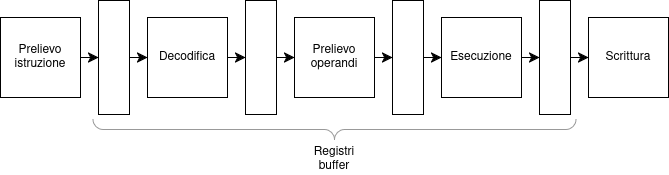
\includegraphics[scale=0.6]{../figures/pipeline.png}
\end{center}
Di base, questa configurazione risulterà comunque un'accelerazione del clock.
Infatti, se l'intera pipeline richiedeva prima un tempo $\Delta$, ci aspettiamo che ogni componente in cui la dividiamo richieda un tempo nell'ordine di $\sim \frac{\Delta}{5}$, ed esattamente $\frac{\Delta}{5}$ se ogni circuiteria ha lo stesso tempo di attraversamento, per cui il clock può essere accelerato di un fattore di $5$.

Il bottleneck è però chiaro per la fase di esecuzione, che potrebbe andare dalla somma naturale alla divisione in virgola mobile, con evidenti differenze in tempo di esecuzione.

Inoltre, la stessa fase di prelievo potrebbe variare in requisiti temporali per via del tipo di codifica delle istruzioni, a lunghezza variabile, adottata dai processori Intel x86 (instruction set \textbf{CISC}, \textit{Complex Instruction Set Computer}, contro gli instruction set \textbf{RISC}, \textit{Reduced Instruction Set Computer}, adottati da ARM).

Ci troveremo quindi di fronte a situazioni dove, con una sola circuiteria di prelievo, non si può sapere quando un'istruzione è veramente finita prima di decodificarla, e quindi non si può procedere con una nuova fase di prelievo.

Chiaramente, tutto questo procedimento è semplificato per i processori ad architettura RISC, in quanto la dimensione delle istruzioni è standardizzata.
Inoltre, si ottengono vantaggi nella gestione della pipeline eliminando la possibilità di avere operandi in memoria: si dedicano istruzioni dedicate alla lettura/scrittura in memoria da registri, cioe le \lstinline|LOAD| e \lstinline|STORE|, più semplici da gestire. 

\subsubsection{Alee}

Altri problemi sono dati dalle \textbf{alee}, cioè legati ai salti condizionali (\textit{alee di controllo}), o a casi dove istruzioni hanno bisogno di risultati di istruzioni ancora in pipeline (\textit{alee di dati}), se non a casi dove la pipeline non permette in primo luogo l'esecuzione successiva di due istruzioni (\textit{alee strutturali}).

\begin{itemize}
	\item 
		Questi problemi possono sempre essere risolti dall'introduzione di \textbf{bolle}: si modificano i registri intermedi perché possano conservare il loro stato, e in caso una certa rete di controllo rilevi situazioni a rischio di alee, si introducono nella pipeline \textit{bolle}, cioè si lasciano stadi di elaborazione vuoti, o se vogliamo si introducono istruzioni \lstinline|nop|, a effetto nullo (che chiaramente rappresentano throughput spreacto).
		I registri che alimentano gli stadi rimasti in attesa manterranno quindi una copia dell'istruzione allo scorso ciclo di clock, e invieranno invece avanti istruzioni nulle.
		In questo modo si torna effettivamente al processore prima della pipeline.
	\item 
		Un'altra soluzione per alee dati e alee strutturali può essere quella di dotare l'ultima fase della pipeline di una linea di \textbf{bypass}, che porti il risultato a termine esecuzione a fronte della fase di esecuzione: un istruzione che richiede un operando non ancora scritto dall'istruzione precedente può ottenerlo direttamente da questa, attraverso il bypass.

	\item 
		Per la gestione delle alee di controllo possiamo sfruttare la cosiddetta \textit{esecuzione predittiva}, in particolare \textbf{branch prediction}: si fa un ipotesi sul risultato dell'istruzione di salto condizionale, e si riempie la pipeline con istruzioni che provengono dalla regione corrispondente di programma.
		Al momento della fase di esecuzione dell'istruzione di salto, si capisce quindi se l'ipotesi si è avverata o meno, e si procede ripulendola completamente introducendo bolle (in caso di \textit{miss}, pagando un prezzo pari al numero di fasi della pipeline) o non facendo nulla (in caso di \textit{hit}).

		Esistono politiche leggermente diverse in caso di salti \textbf{diretti} (con indirizzo noto) o \textbf{indiretti} (ad indirizzi calcolati).

		\begin{itemize}
			\item 
				\textbf{Salti diretti}: in questo caso si fa una predizione \textbf{statica}, cioè si sceglie sostanzialmente a caso fra gli esiti del salto.
				Esistono comunque alcune euristiche che possiamo usare: nel caso di salti \textit{all'indietro} ci si aspetta di entrare in un loop, e quindi si assume che il salto verrà eseguito; di contro per salti \textit{in avanti} l'ipotesi è meno forte e ci si aspetta che il salto non verrà eseguito. 

				\newpage

				Abbiamo quindi a grandi linee la struttura funzionale:
				\begin{center}
					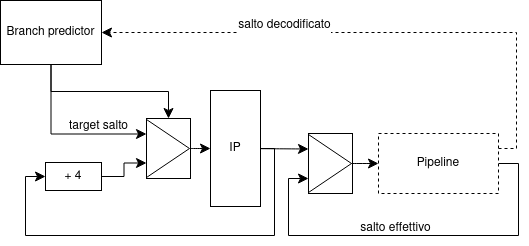
\includegraphics[scale=.65]{../figures/branch_static.png}
				\end{center}
				dove una qualche rete di branch prediction valuta le regole appena valutate per ogni istruzione di salto decodificata dalla pipeline, e invia al primo stadio della pipeline stessa la prossima istruzione che ne ricava. 
				Notiamo che il $+4$ corrisponde al calcolo dell'indirizzo della prossima istruzione sequenziale: si assume che l'architettura abbia istruzioni RISC fisse a 4 byte (vedremo che nelle architetture moderne la semplificazione non è inopportuna).

			\item 
				\textbf{Salti indiretti:} Per questi ci si aspetta che i salti si comporteranno come si sono comportati in precedenza, cioè si fa una predizione \textbf{dinamica}.
				Questo compito è associato ad una componente detta \textbf{BTB}, \textit{Branch Target Buffer}, che si occupa di capire se un salto verrà effettuato o meno sulla base della sua storia precedente, e a quale locazione si salterà, sempre basandosi sulla storia precedente, nel caso di salti indiretti.

				Questi circuiti assumono essenzialmente la forma di cache, e visto che il loro insuccesso (\textit{miss}) risulta solo in un annullamento di un ciclo di pipeline, non si preoccupano di gestire le collisioni.

				In questo caso la struttura funzionale è del tipo:
				\begin{center}
					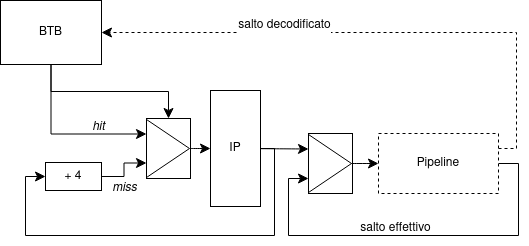
\includegraphics[scale=.65]{../figures/branch_dynamic.png}
				\end{center}
				cioè sostanzialmente analoga alla precedente ma dove l'ipotesi sul prossimo salto viene fatta dall'hit/miss della cache BTB.

Si ha che nelle architetture moderne l'approccio adottato effettivamente è quello del BTB, sia per i salti diretti che i salti indiretti.
Chiaramente ci saranno differenze strutturali specifiche per le informazioni che sarà necessario memorizzare per entrambi i tipi di salto: se per i salti indiretti è fondamentale ricordare l'indirizzo di arrivo, per i salti diretti basterà ricordare se il salto è stato effettuato o meno.
In ogni caso, può essere utile conservare anche l'indirizzo di arrivo per questioni di ottimizzazione: l'indirizzo potrebbe sì essere ricavato dall'istruzione, ma questo richiederebbe la sua decodifica, mentre il prefetch può iniziare prima ricavando l'indirizzo di arrivo direttamente dall'indirizzod dell'istruzione.
		\end{itemize}

\end{itemize}

\subsubsection{Architettura del Pentium Pro}
Nei processori di oggi, la gestione della pipeline è effettivamente quella che Intel sviluppa dal Pentium Pro del 1995 (che ha continuato ad evolvere fino ad oggi, se non per una deviazione che fu esplorata nel Pentium 4).

In questa architettura, il processore si occupa di tradurre intermante le istruzioni CISC in istruzioni RISC, e quindi a gestire la pipeline con sole istruzioni RISC.
Vorremo quindi rimuovere le fasi di prelievo e decodifica dalla pipeline vista finora, per porle esternamente come parte del ciclo di traduzione da CISC a RISC, e aspettarci che la pipeline vera e propria si veda arrivare istruzioni già decodificate. 

\par\medskip

Notiamo infine che spesso nemmeno l'esecuzione sequenziale del codice non è necessaria.
Prendendo ad esempio il frammento di codice:
\begin{lstlisting}[language=C++, style=codestyle]	
for(int i = 0; i < 1000; i++) {
	a[i] = v1[i] * v2[i];
}
\end{lstlisting}
potremmo "srotolarlo" in:
\begin{lstlisting}[language=C++, style=codestyle]	
a[0] = v1[0] * v2[0];
a[1] = v1[1] * v2[1];
// ...
a[999] = v1[999] * v2[999];
\end{lstlisting}

\subsubsection{Esecuzione asincrona}
Vediamo che nessuna di queste istruzioni dipende dalle altre, ergo l'ordine in cui vengono eseguite non è importante.
In questo caso il miss di cache per alcune di queste può tradursi semplicemente in un ritardo nella loro esecuzione, mentre altre che invece si trovano in cache (magari relative ad indirizzi successivi) possono essere eseguite da subito, cioè l'esecuzione asincrona è non solo possibile, ma può risultare anche utile.

\subsubsection{Esecuzione predittiva}
Un'ultima tecnica che il processore moderno può usare per accelerare l'esecuzione delle istruzioni è eseguire istruzioni prima che questo sia necessario, eventualmente scartando i risultati nel caso risultino inutili. 

\end{document}
